\subsubsection{Squat}

The squat is the first of the three lifts in a competition, and is a movement in which the legs are the main driving force. The barbell is placed on the lifter’s shoulders, and the lifter must bend at their knees and hip to bring their hip joint below their knees. When they have reached this position, they must then push hard with their legs to return to an upright position. Figure~\ref{fig:squat_stages} shows an example of a squat.

\begin{figure}[H]
    \centering
    \subfigure[Begin]{
            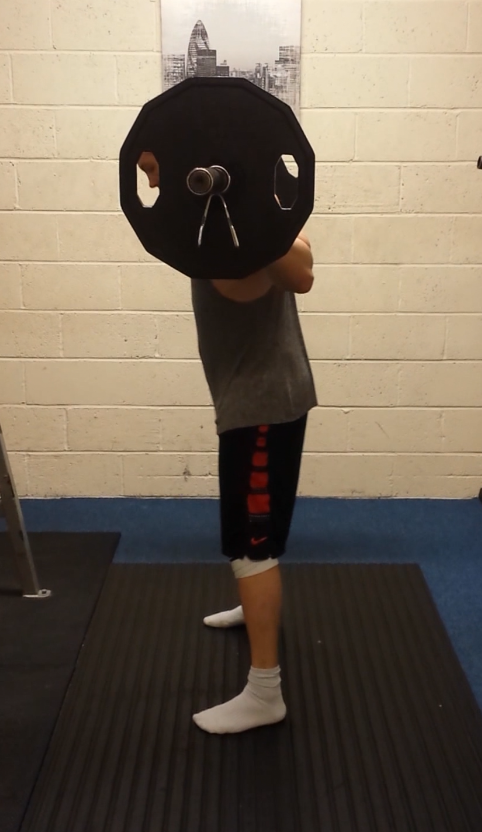
\includegraphics[height= 7cm]{intro/images/squat_start}
    }
    \subfigure[Middle]{
            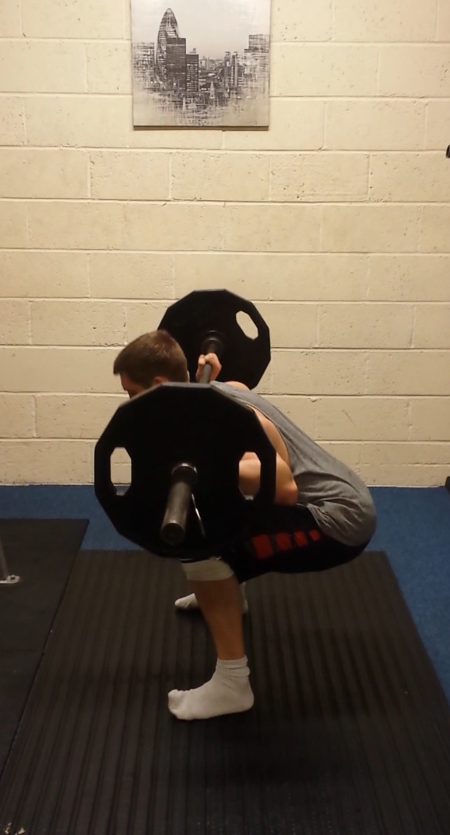
\includegraphics[height= 7cm]{intro/images/squat_middle}
    }
    \subfigure[End]{
            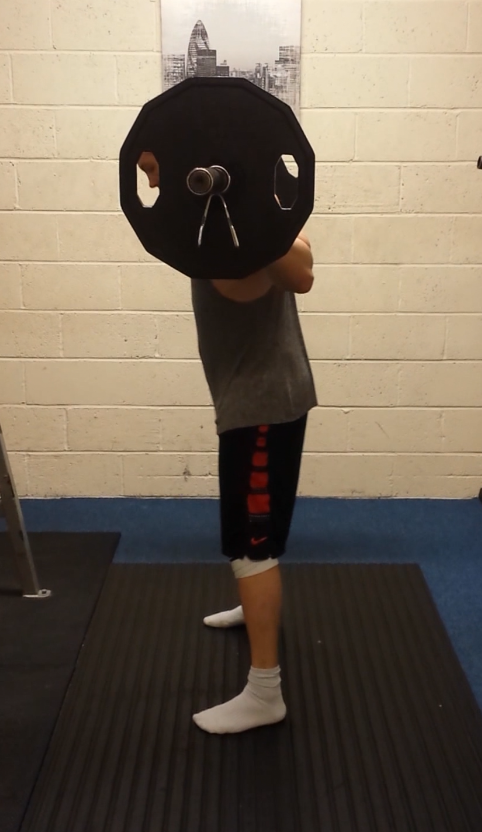
\includegraphics[height= 7cm]{intro/images/squat_start}
    }
\caption{The stages of a squat}
\label{fig:squat_stages}
\end{figure}

The International Powerlifting Federation regulations\cite{ipf} give a list of the criteria used to deem whether a lift is successful or not. In competition, the main objective is to reach sufficient depth and return to the upright position with no external help. In addition, when the lifter has started their ascent, there must be no further downward movement. In training, it is considered good practice for a lifter to keep their shins perpendicular to the ground in order to minimise the risk of knee injury. It is also advantageous for the lifter to keep the bar directly above their feet at all times during the lift, establishing a better position to drive the bar upwards.